\documentclass[10pt]{beamer}

\usepackage{amssymb}
\usepackage{latexsym}
\usepackage{amsmath}

\usepackage{verbatim}
\usepackage{algorithm}
\usepackage[noend]{algorithmic}
\usepackage{graphicx}
\usepackage{xcolor}
\usepackage{epsfig}
\usepackage[noend]{algorithmic}
\usepackage{graphicx}
\usepackage{xcolor}
\usepackage{epsfig}
\usepackage{synttree}
\usepackage{ulsy}
\usepackage{multicol}
\usepackage[english]{babel}
\usepackage{media9}
\usepackage{epsfig}
\usepackage{epstopdf}
\usepackage{accents}
\usepackage{hyperref}
\usepackage{times}
\usepackage[T1]{fontenc}
\usepackage{multimedia}

\usetheme{Warsaw}
%\usecolortheme{albatross}
%\definecolor{red}{RGB}{47,88,55} % use structure theme to change
%\definecolor{c_ltgreen}{RGB}{81,127,90}
%\definecolor{c_dkgreen}{RGB}{12,49,19}
%\definecolor{c_cream}{RGB}{248,245,234}

%\setbeamercolor*{palette secondary}{bg=c_ltgreen}
%\setbeamercolor*{palette primary}{fg=c_cream, bg=c_dkgreen}
%\setbeamercolor*{palette tertiary}{fg=c_cream, bg=c_green}

%\setbeamercolor{author}{parent=palette tertiary}
%\setbeamercolor{frametitle}{parent=palette secondary}
%\setbeamercolor{structure}{fg=c_cream,bg=c_dkgreen}

\newcommand{\N}{\mathbb{N}}
\newcommand{\Z}{\mathbb{Z}}
\newcommand{\C}{\mathbb{C}}
\newcommand{\R}{\mathbb{R}}
\renewcommand{\d}{\ensuremath{\diamond}}
\newcommand{\DOL}{\ensuremath{\theta ^\omega (a)}}
\newcommand{\HDOL}{\ensuremath{\varphi \circ \theta ^\omega(a)}}
\newcommand{\pababa}{\ensuremath{\alpha \beta \alpha \beta \alpha}}


\title{Wavelet-Based Compression of Signals}
\author{ Shane Scott }
\date{\today}
\institute{Kansas State University}

\newtheorem{conjecture}{Conjecture}
\newtheorem{proposition}{Proposition}
\newtheorem{remark}{Remark}

\begin{document}

\begin{frame}
\titlepage
\end{frame}

\begin{frame}
\frametitle{Hilbert Spaces}
\begin{block}
{Signals} Signals are vectors in the Hilbert space
$$
L_2 = \left \{ v: \R \to \C \  \middle | \ \int_\R |v(t)|^2 dt \right \}
$$
\end{block}
\pause
\begin{block}
{Digital Signals}
In practice we typically use \emph{digital signals} in the Hilbert space 
$$
\ell_2\Z_N = \left \{ z: \Z_N \to \C  \right \}
$$
\end{block}
\end{frame}

\begin{frame}
\frametitle{Hilbert Spaces}
\begin{block}
{Inner Product} Hilbert spaces are equipped with the inner product $\langle \cdot | \cdot \rangle: H \times H \to \C$. For $L_2$
$$
\langle u|v\rangle= \int_\R \overline{u(t)}v(t) dt
$$
\pause or for $\ell_2 \Z_N$
$$
\langle u|v\rangle = \sum^{N-1}_{k=0} \overline{u_k}{v_k}
$$
\pause and are Cauchy complete with respect the the metric/norm
$$
\|u-v\|=\langle u-v|u-v \rangle^\frac{1}{2}
$$
\end{block}
\end{frame}

\begin{frame}
\frametitle{Hilbert Spaces}
\begin{block}
{Bases}
If $\{a_k | k \in \Z\}$ is a complete othonormal basis for a Hilbert space $H$ then any $v \in H$ can be written in the form
$$
v=\sum_{k \in \Z} \langle a_k|v \rangle a_k
$$
\end{block}
\end{frame}

\begin{frame}
\frametitle{Fourier Transform}
\begin{block}
{Fourier Transform}
If $f \in L_2$ we call its Fourier transform $\hat f$ the function
$$
\hat f (\omega)= \frac 1 {\sqrt{2\pi}}\int_\R f(t)e^{-it\omega} dx
$$
(when it exists). \pause Theres an inverse
$$
f(t)=(\hat f )^\vee (t)= \frac 1 {\sqrt{2\pi}}\int_\R \hat f(\omega)e^{it\omega} d\omega
$$
\pause That is (almost)
$$
f(t)=\int_\R \langle \frac{e^{it\omega}}{\sqrt{2\pi}} |f\rangle \frac{e^{it\omega}}{\sqrt{2\pi}} d\omega
$$
\end{block}
\end{frame}

\begin{frame}
\frametitle{Fourier Transform}
\begin{block}
{Fourier Transform}
If $z \in \ell_2\Z_N$ we call its Fourier transform $\hat z$
$$
\hat z_m= \sum^{N-1}_{n=0} z_n \frac{e^{-i2\pi mn/N}}{\sqrt N}
$$
\pause We have
$$
z_n= \sum^{N-1}_{m=0} \langle \frac{e^{i2\pi mn/N}}{\sqrt N} | z \rangle \frac{e^{i2\pi mn/N}}{\sqrt N}
$$
\end{block}
\end{frame}

\begin{frame}
\frametitle{The Walken Signal z}
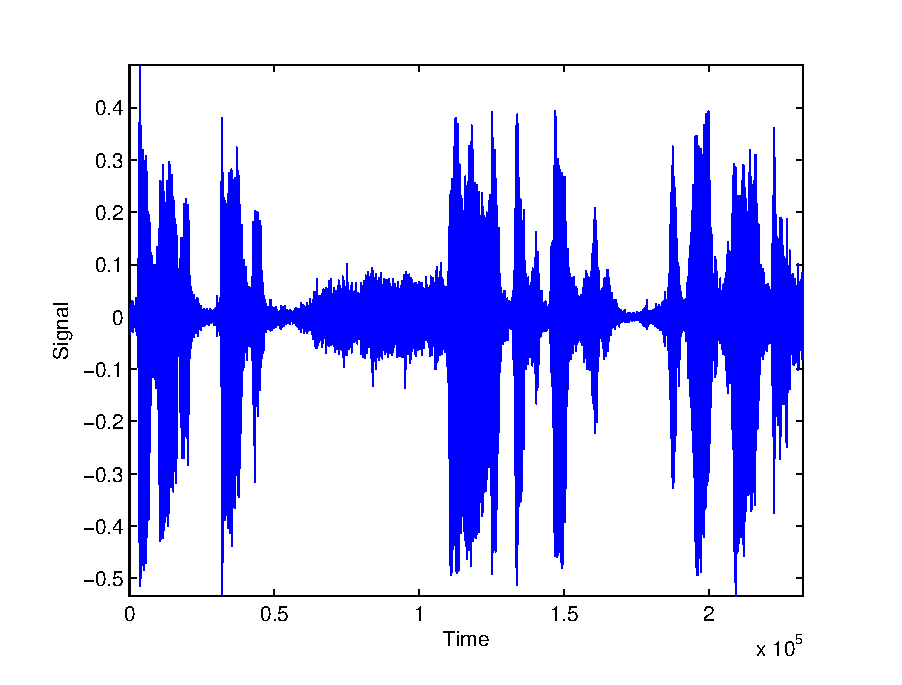
\includegraphics[height=8cm]{figure1.eps}
\movie[inlinesound]{\fbox{Play}}{igottafever.wav}%{floaton.mpg}
\includemedia[flashvars={source=igottafever.wav}]{\fbox{Play}}{APlayer.swf}%{floaton.mpg}
\end{frame}

\begin{frame}
\frametitle{Fourier Compression}
\begin{block}
{An easy low-loss compression}
Discard the lowest $p^{th}$ percent of Fourier coefficients, replacing them by zero.
\end{block}
\end{frame}

\begin{frame}
\frametitle{$\hat z$ The Walken Spectrum (Fourier Transform)}
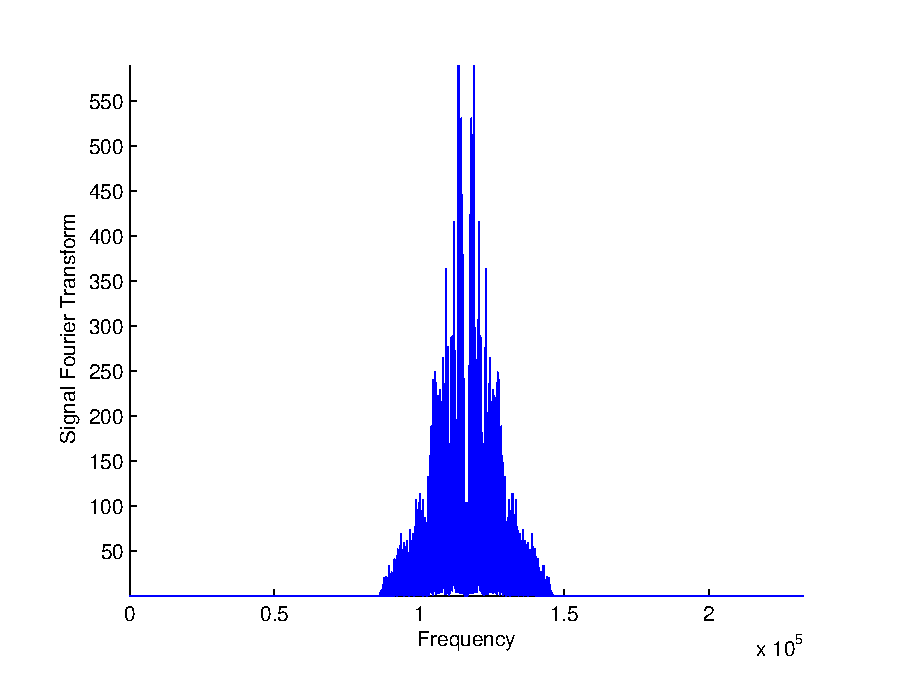
\includegraphics[height=8cm]{Fourier.eps}
\end{frame}

\begin{frame}
\frametitle{$\hat z$ The Walken Spectrum 90\% Compressed}
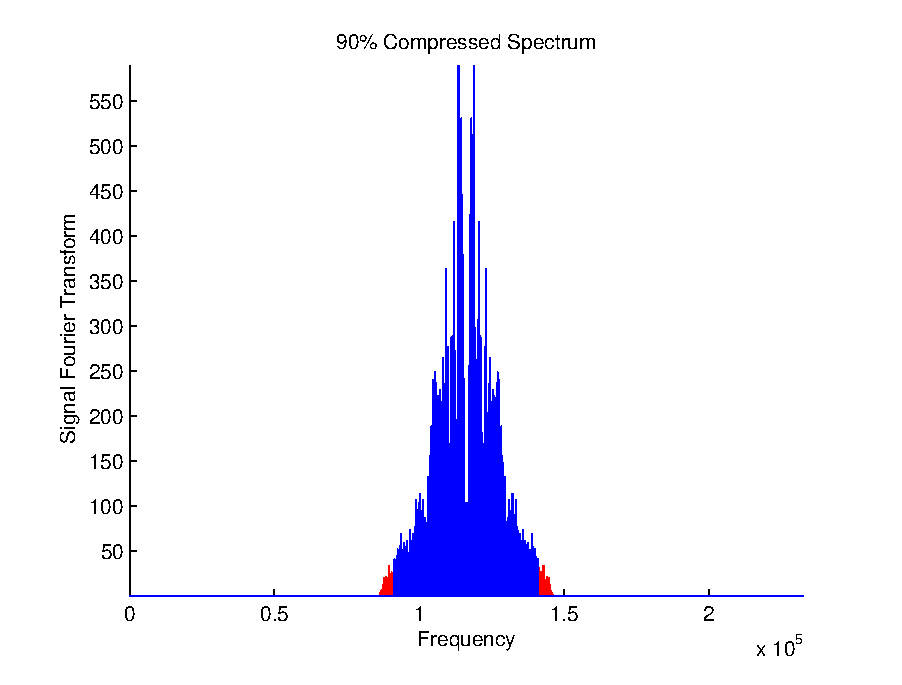
\includegraphics[height=8cm]{90four.eps}
\end{frame}

\begin{frame}
\frametitle{$z$ The Walken Signal 90\% Compressed}
\movie[inline]{\fbox{Play}}{90Fourier.wav}%{floaton.mpg}
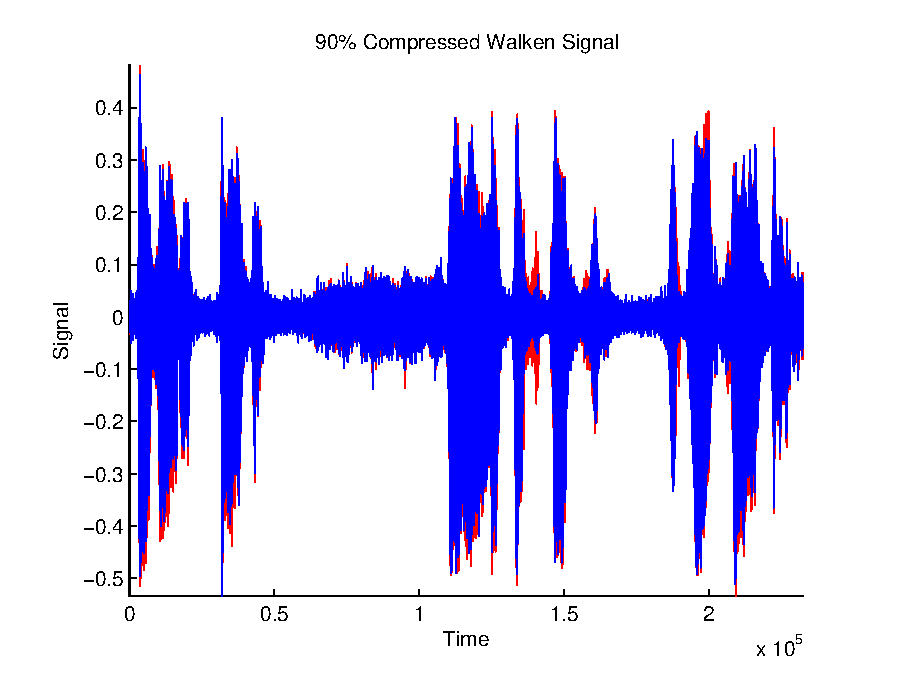
\includegraphics[height=7.5cm]{90fourRec.eps}
\end{frame}


\begin{frame}
\frametitle{$\hat z$ The Walken Spectrum 95\% Compressed}
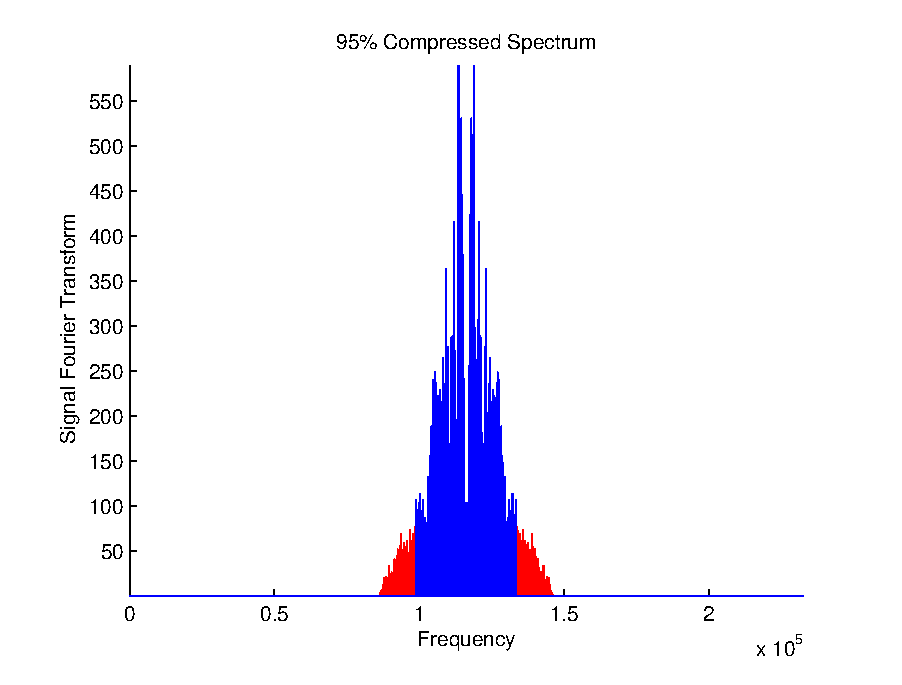
\includegraphics[height=8cm]{95four.eps}
\end{frame}

\begin{frame}
\frametitle{$z$ The Walken Signal 95\% Compressed}
\movie[inline]{\fbox{Play}}{95Fourier.wav}%{floaton.mpg}
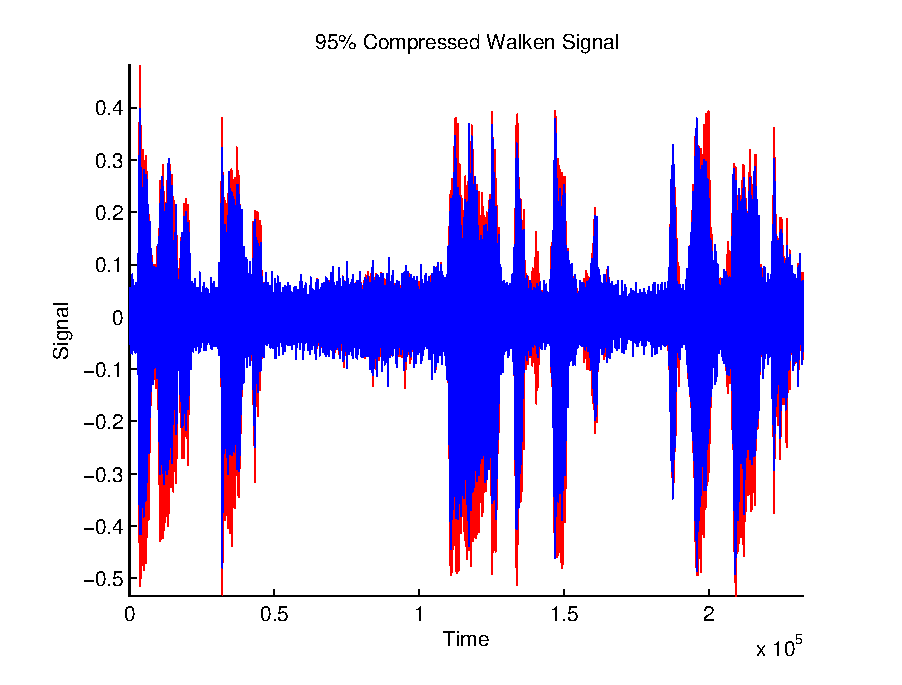
\includegraphics[height=7.5cm]{95fourRec.eps}
\end{frame}

\begin{frame}
\frametitle{Problems}
\begin{block}{Practial Objection}
$$
z_n=\sum^{N-1}_{m=0} \hat z_m \frac{e^{i2\pi mn/N}}{\sqrt N}
$$
$$
f(t)=\int^\infty_{-\infty} \hat f (\omega)  \frac{e^{it\omega}}{\sqrt{2\pi}}d\omega
$$
Delocalization
\begin{enumerate}
\item Signal is delocalized in \emph{frequency} space
\item Spectrum is delocalized in \emph{temporal} space
\end{enumerate}
\end{block}
\end{frame}

\begin{frame}
\frametitle{Localization in Streaming}
\center
\includemedia[
	deactivate=pageclose,
	width=200pt, height=150pt,
	addresource=walkenclip.mp4,
	flashvars={src=walkenclip.mp4 & loop=false &autoPlay=true}
]{\fbox{Play}}
{StrobeMediaPlayback.swf}
\end{frame}

\begin{frame}
\frametitle{Problems}
\begin{block}{Practial Objection}
$$
z_n=\sum^{N-1}_{m=0} \hat z_m \frac{e^{i2\pi mn/N}}{\sqrt N}
$$
$$
f(t)=\int^\infty_{-\infty} \hat f (\omega)  \frac{e^{it\omega}}{\sqrt{2\pi}}d\omega
$$
Delocalization
\begin{enumerate}
\item Signal is delocalized in \emph{frequency} space
\item Spectrum is delocalized in \emph{temporal} space
\end{enumerate}
\end{block}
\pause
\begin{block}
{Impractical Objection}
$$
\frac{e^{it\omega}}{\sqrt{2\pi}} \notin L_2
$$
This isn't a basis for $L_2$.
\end{block}
\end{frame}

\begin{frame}
\frametitle{Wavelets}
\begin{block}{Wavelets in $L_2$}
A wavelet in $L_2$ is $\psi \in L_2$ such that
$$
\psi_{j,k}(t)=2^{j/2}\psi(2^jt-k)
$$
satisfy $\left \{\psi_{j,k} \ \middle | \ j,k \in \Z \right \}$ is a complete, orthonormal basis.
\end{block}
\end{frame}

\begin{frame}
\frametitle{Mexican Hat Wavelet}
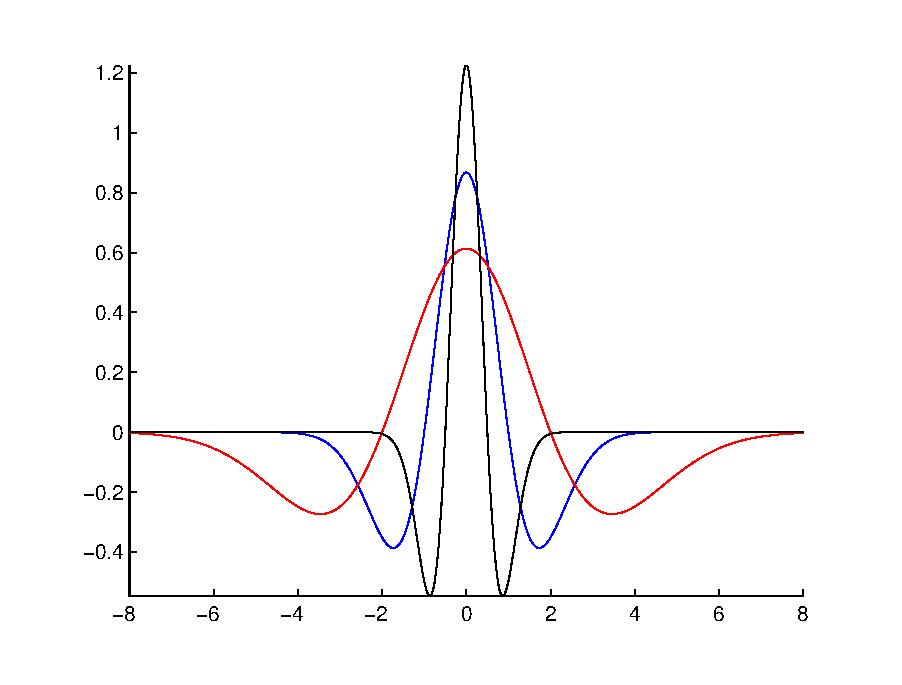
\includegraphics[height=8cm]{mexhats.eps}
\end{frame}

\begin{frame}
\frametitle{Mexican Hat Fourier Transform}
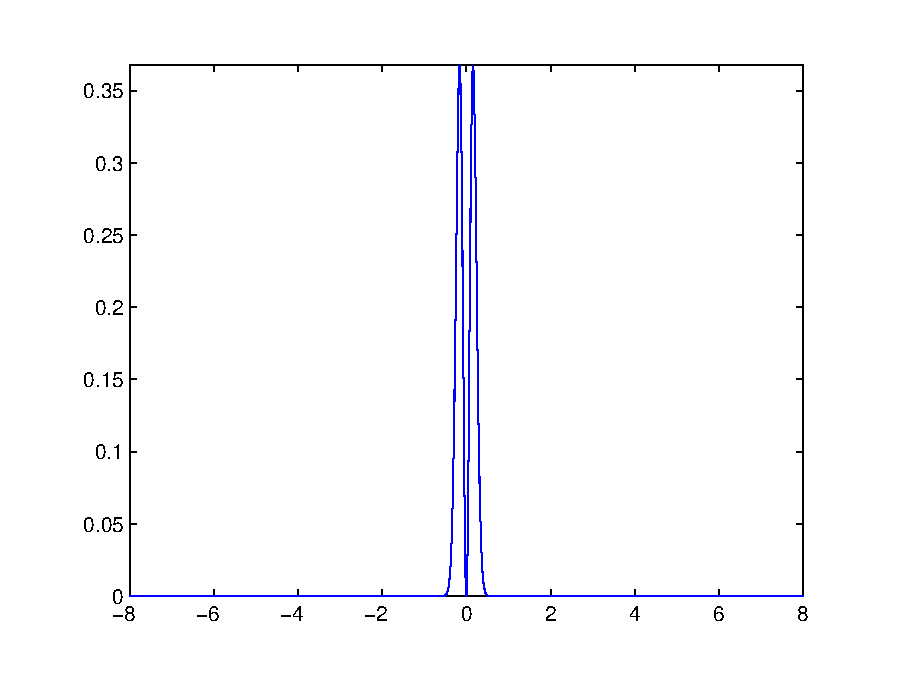
\includegraphics[height=8cm]{mexhatFour.eps}
\end{frame}

\begin{frame}
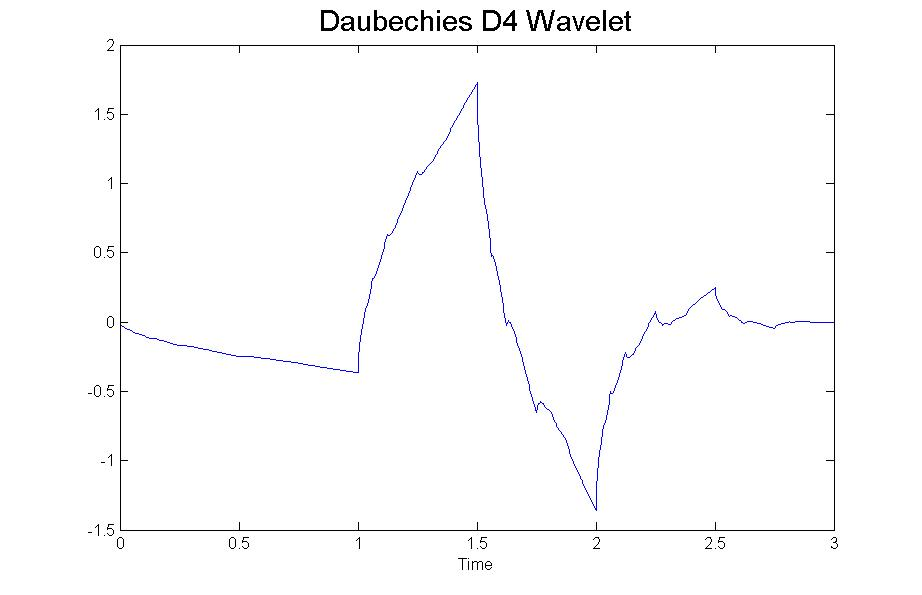
\includegraphics[height=8cm]{D4}
\end{frame}

\begin{frame}
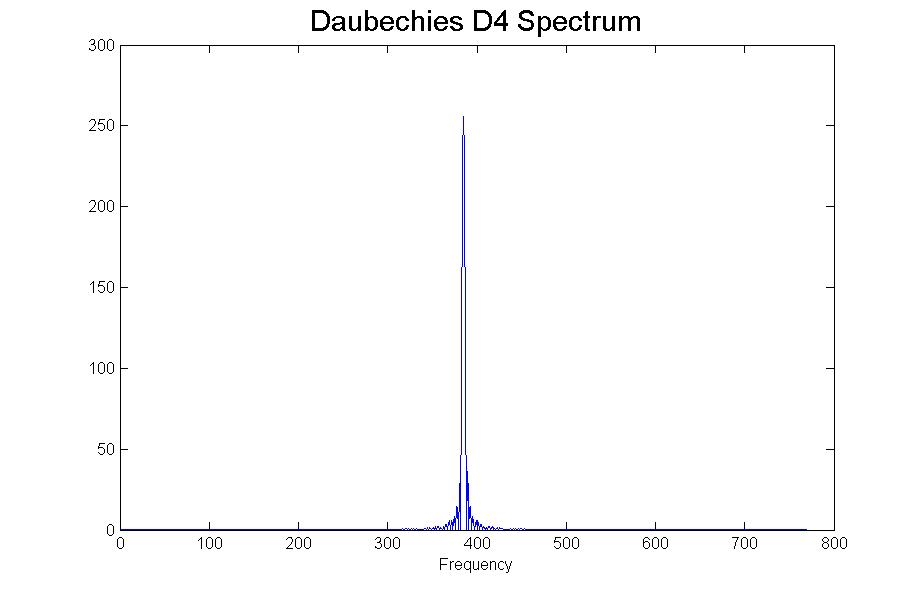
\includegraphics[height=8cm]{D4Spec}
\end{frame}

\begin{frame}
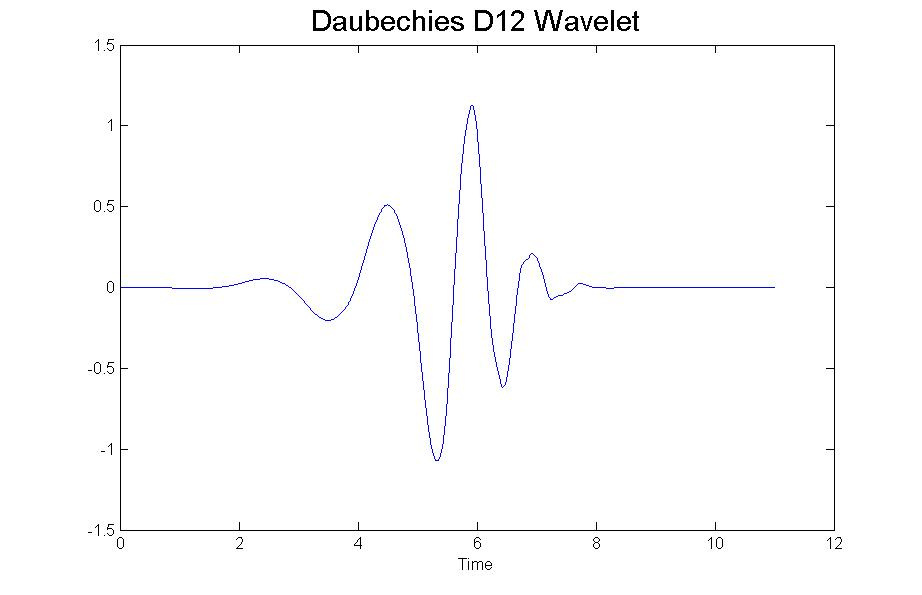
\includegraphics[height=8cm]{D12}
\end{frame}

\begin{frame}
\includegraphics[height=8cm]{D12Spec}
\end{frame}

\begin{frame}
\frametitle{Wavelets}
\begin{block}{$k^{th}$ Translation}
If $z\in \ell_2 \Z_N$
$$
R_k z_n=z_{n-k}
$$
\end{block}
\begin{block}{Wavelets in $\ell_2 \Z_N$}
A first stage wavelet pair is a pair of vectos $u,v \in \ell_2 \Z_N$ such that
$$
B= \{ R_{2k}u \ | \ k=0,\ldots,N/2-1 \} \cup \{ R_{2k}v \ | \ k=0,\ldots,N/2-1 \}
$$
is a complete othonormal basis fo $\ell_2 \Z_N$
\end{block}
\end{frame}

\begin{frame}
\frametitle{Wavelets}
\begin{block}{Low Pass and High Pass}
A wavelet pair $u,v$ must satisfy
$$
|\hat u(n)|^2+|\hat u(n+N/2)|^2=2
$$
\begin{enumerate}
\item \pause Put $\hat u (0)=\sqrt 2$ and $\hat u (N/2)=0$, $u$ is the \emph{low pass filter}
\item \pause Put $\hat v (N/2)=\sqrt 2$ and $\hat v (0)=0$, $v$ is the \emph{high pass filter}
\end{enumerate}
\end{block}
\begin{block}
{z expansion}
$$
z=\sum_{n=0}^{N/2-1}\langle R_{2k}u|z \rangle  R_{2k}u+\sum_{n=0}^{N/2-1}\langle R_{2k}v|z \rangle  R_{2k}v
$$
\begin{enumerate}
\item \pause The first term contains an approximation.
\item \pause The second term contains the details.
\end{enumerate}
\end{block}
\end{frame}

\begin{frame}
\includegraphics[height=6.5cm]{d4Pair}
\end{frame}

\begin{frame}
\frametitle{The Walken Signal}
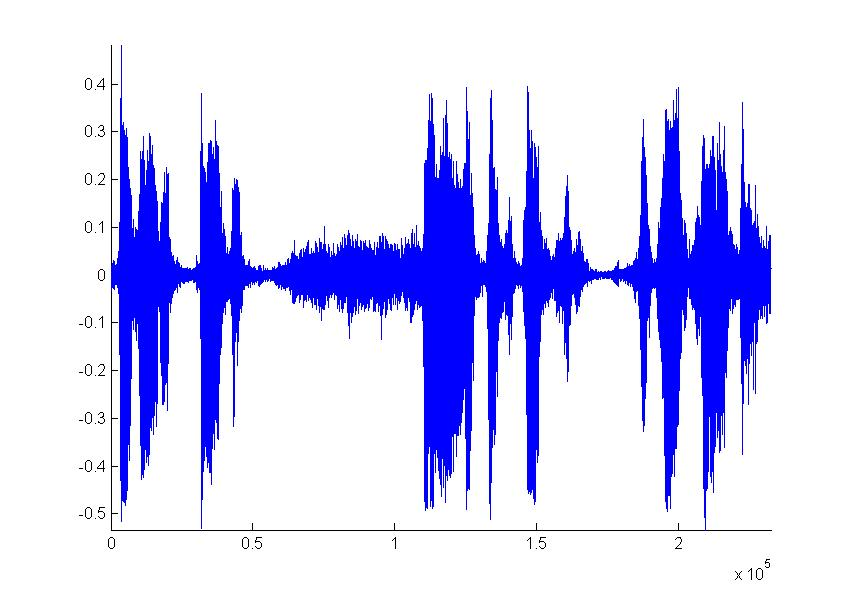
\includegraphics[height=7cm]{stage0}
\end{frame}

\begin{frame}
\frametitle{1st Stage Wavelet Representation}
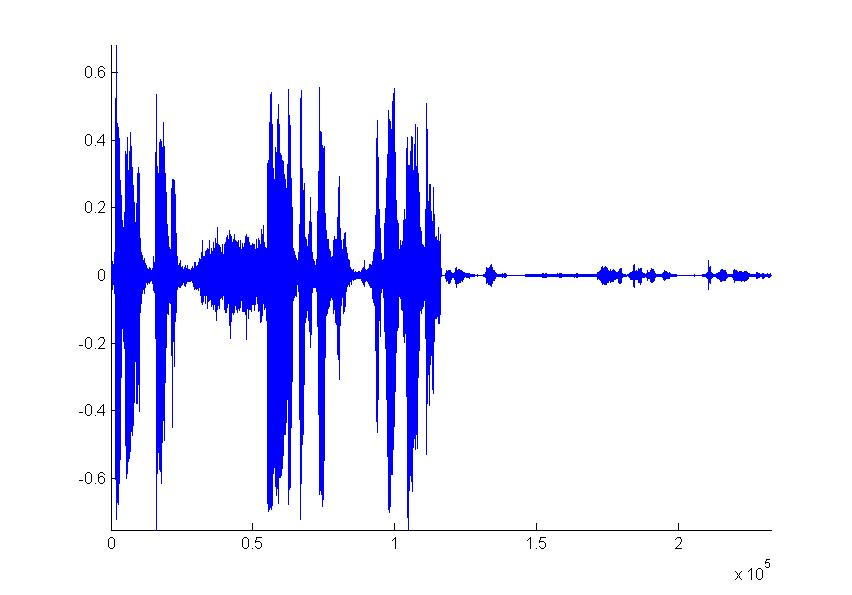
\includegraphics[height=7cm]{stage1}
\end{frame}

\begin{frame}
\frametitle{2nd Stage Wavelet Representation}
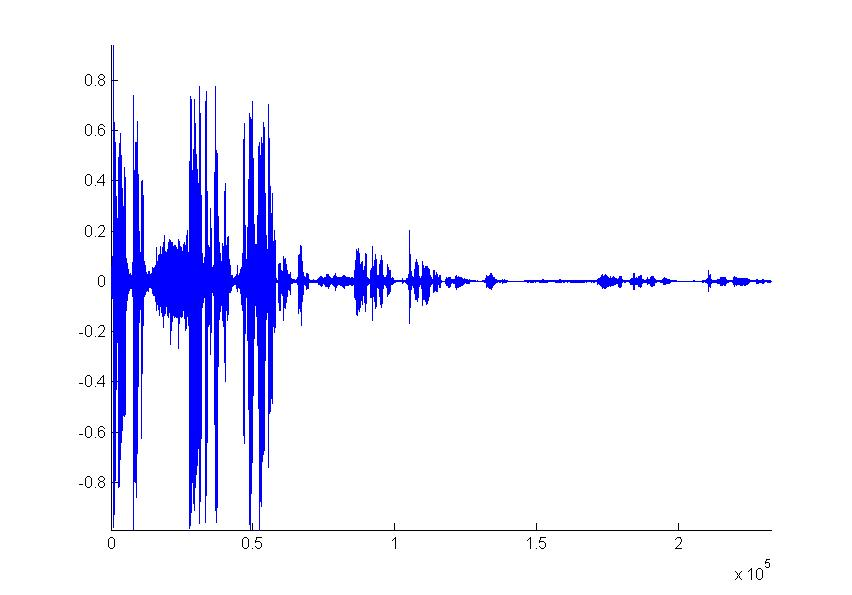
\includegraphics[height=7cm]{stage2}
\end{frame}

\begin{frame}
\frametitle{3rd Stage Wavelet Representation}
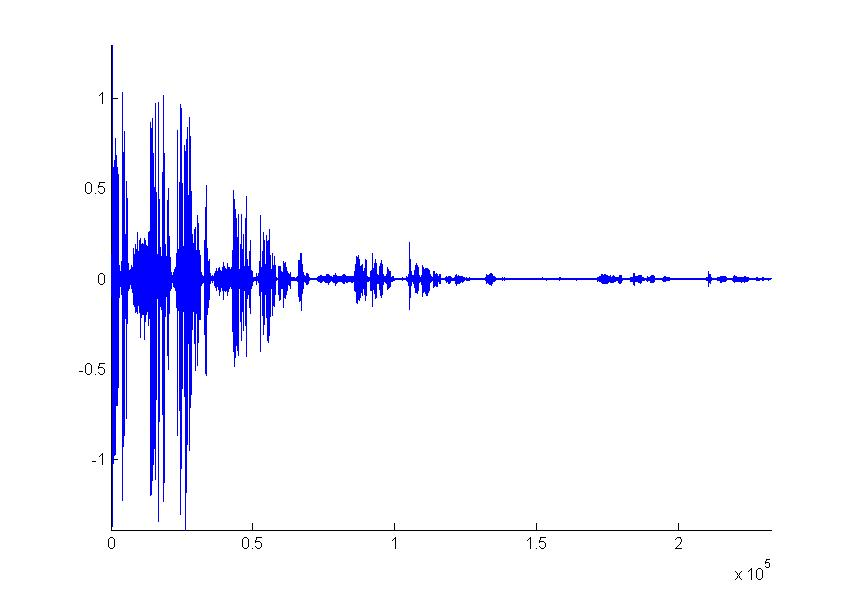
\includegraphics[height=7cm]{stage3}
\end{frame}

\begin{frame}
\frametitle{4th Stage Wavelet Representation}
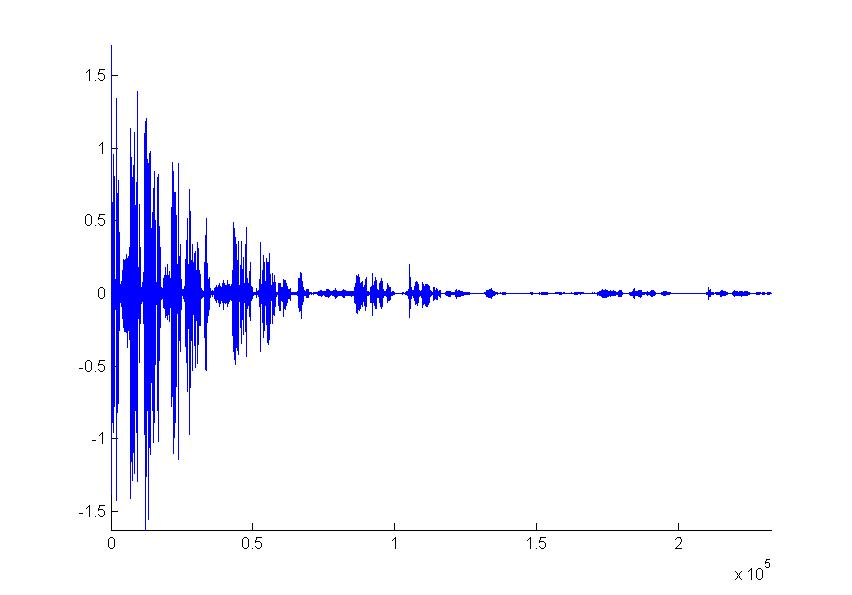
\includegraphics[height=7cm]{stage4}
\end{frame}

\begin{frame}
\frametitle{4th Stage Wavelet Representation 90\% Compression}
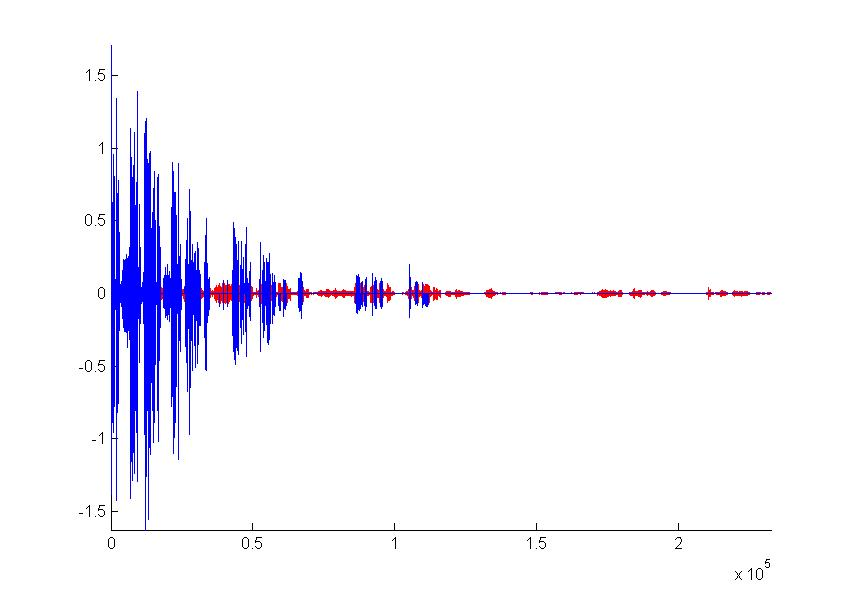
\includegraphics[height=7cm]{stage4p9}
\end{frame}

\begin{frame}
\frametitle{Reconstructed 90\% Compression}
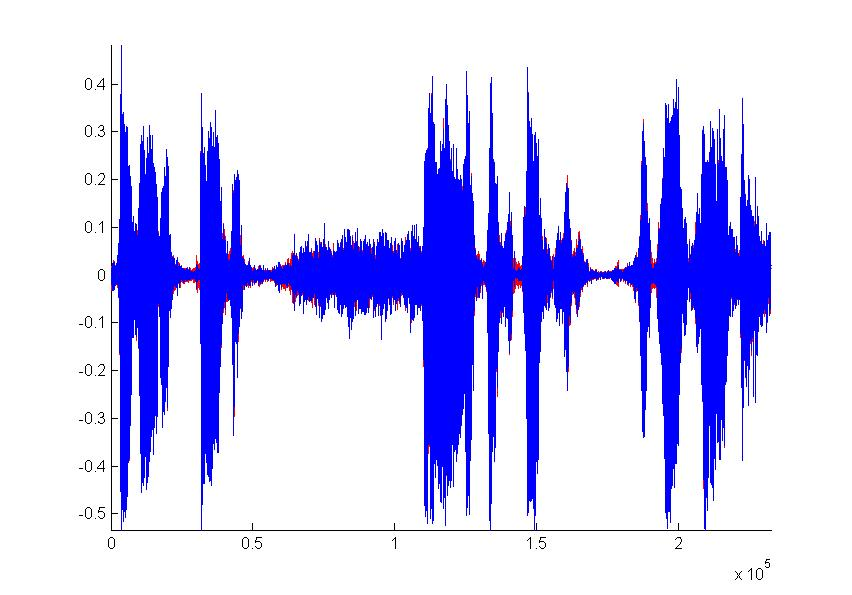
\includegraphics[height=7cm]{reConstructp9}
\movie[inline]{\fbox{Play}}{90D4.wav}%{floaton.mpg}
\end{frame}

\begin{frame}
\frametitle{5th Stage Wavelet Representation  95\% Compression}
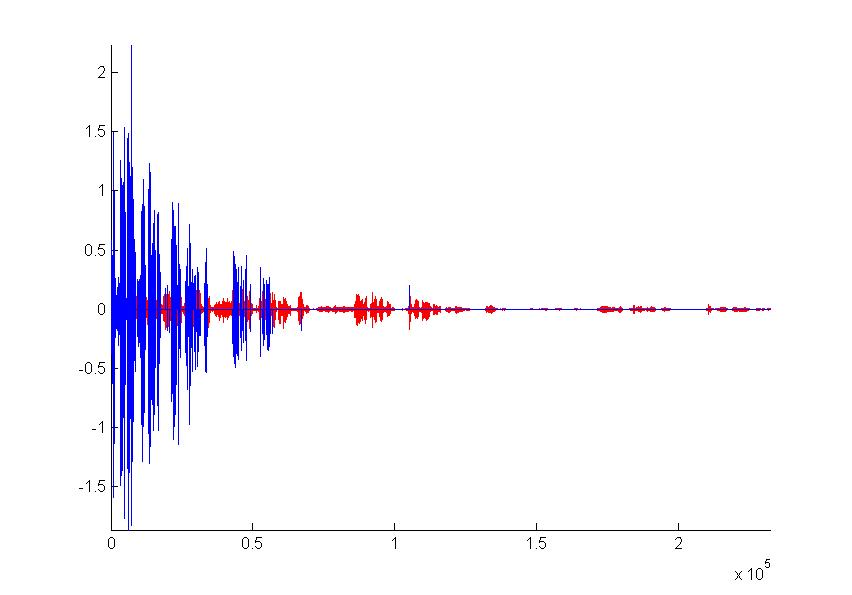
\includegraphics[height=7cm]{stage4p95}
\end{frame}

\begin{frame}
\frametitle{Reconstructed 95\% Compression}
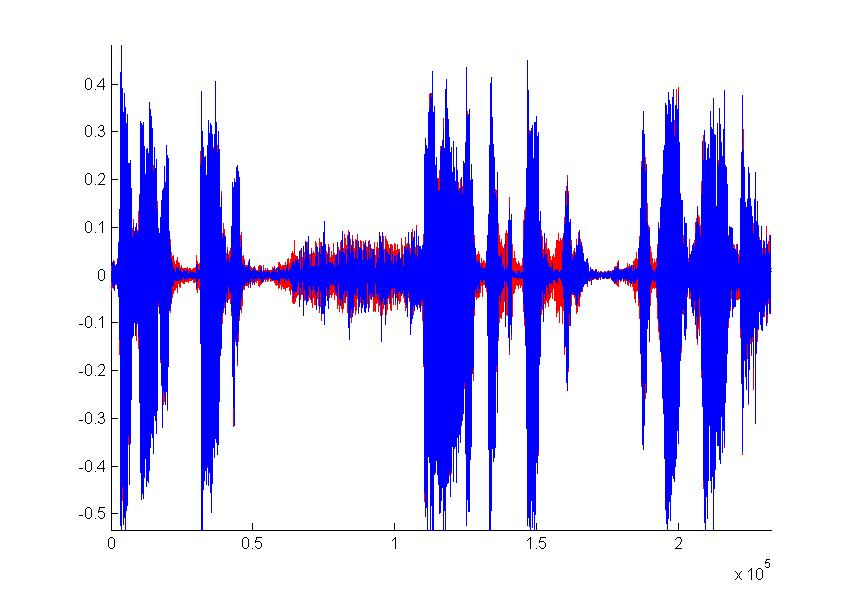
\includegraphics[height=7cm]{reConstructp95}
\movie[inline]{\fbox{Play}}{95D4.wav}%{floaton.mpg}
\end{frame}

\begin{frame}
\frametitle{Sound Comparison}
\movie[inline]{\fbox{Original}}{igottafever.wav}\\
\movie[inline]{\fbox{.9 Compressed Fourier}}{90Fourier.wav}\\%{floaton.mpg}
\movie[inline]{\fbox{.95 Compressed Fourier}}{95Fourier.wav}\\%{floaton.mpg}
\movie[inline]{\fbox{.9 Compressed Wavelet}}{90D4.wav}\\%{floaton.mpg}
\movie[inline]{\fbox{.95 Compressed Wavelet}}{95D4.wav}\\%{floaton.mpg}
\end{frame}

\begin{frame}
\frametitle{Percent Error Comparisons}
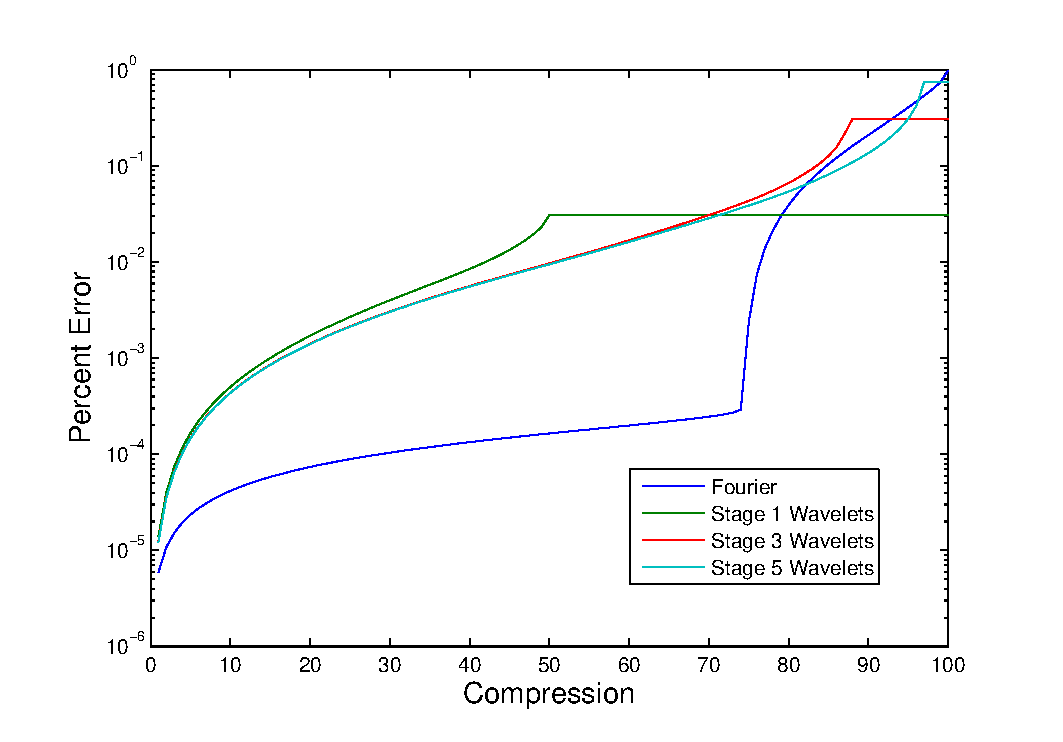
\includegraphics[height=7cm]{error.eps}
\end{frame}

\begin{frame}
\frametitle{Acknowledgments}
\begin{block}{Thank You}
This presentation is based on work with Brian Moore, Vincent Pigno, and Virginia Naibo and supported by the Kansas State University i-Center for the Integration of Undergraduate, Graduate, and Postdoctoral Research.
\end{block}

\includegraphics[height=2cm]{icenterlogo2}
\end{frame}

\end{document}